\chapter{Introduction}
% Needs to lay out the wider story of why seasons are important,
% which becomes a narrative thread throughout the thesis.
% This should answer the `why bother' question, and justify the research.

% Another ongoing thread is `multiple approaches yield richer results'.


This thesis will investigate and characterise an Indigenous seasonal calendar.
I combine Indigenous knowledge with Western climate science to characterise
local seasonality in NE Arnhem Land (see \autoref{fig:arnhem-map}),
as described by a Yolngu seasonal calendar I construct based on
interviews and supported by literature.\\

Previous research has focussed on the social or ecological aspects of Australian
Indigenous calendars.  This thesis instead treats Indigenous knowledge as a
\emph{framework for} research, not simply an \emph{object of} research.
Togther with an interdisciplinary approach quantifying Indigenous seasons,
my results are highly novel -- and indeed, to my knowledge unique.



\section{TODO - Topic Introduction}
Indigenous Seasons and Ecological Knowledge

% - One paragraph on the global-scale reason to care about the topic
% - Lay out how Indigenous seasons are defined (inc. international, contrast)
% - draw link to ecological knowledge
% - Explain shortcomings in existing research



Where Australia's formally recognised seasons are defined by Gregorian date -
e.g. December 1 is by definition the first day of Summer - Indigenous seasons
are defined by weather and ecological events.
%
This more closely matches intuitions about seasons as annually recurring
periods marked by weather - most commonly temperature, which tends to
follow sunlight intensity - than a date-based approach, though Indigenous
seasons are more nuanced than ``hot == summer, cold == winter''.

Like the observation-based approach used in some Nordic nations, where
seasons are defined by persistent temperature change (REF),
Indigenous Australian seasons are recognised after the fact and vary
between years depending on the behaviour of their indicators.


A Yolngu seasonal calendar was chosen as the case study for this thesis
as personal relationships in the region facilitated qualitative research,
and the emphasis on meteorological indicators allows quantification based
on the observational weather record.


There are other `whys'; including proportion of population which is Indigenous,
community engagement in traditional and western land management, etc.


~\\
~\\
Section beyond this point is DRAFT NOTES ONLY


Highly localised.
Yolngu calendars of North-East Arnhem Land divide the year into
six seasons based on prevailing wind, rainfall, temperature,
and a variety of other factors.

Derivation of the seasonal calendar from current conditions,
along with the impossibility of applying the European seasonal calendar
to the tropical seasonality, make Yolngu seasons an excellent case study.

See \citet{menzel2006} re modern scientific use of ecological changes
as indicators of seasonal onset or climate change.



Indigenous knowledge is recognised and valued in an increasing variety
of contexts \citep[eg.][]{petheram2010,cochran2015,berkes2012} –
but integration with the physical sciences is still relatively rare and ad-hoc.
%
I argue that such synthesis provides a crucial long-term perspective on
anthropogenic environmental change, and demonstrate that such synthesis
can produce novel results for both scientific and indigenous stakeholders.

Ecological knowledge is embedded in calendars.




\section{Research Context}
\label{ch:context}
This section lays out the study area and scope of the thesis.

NOTE - needs extensive edits below.\\



\begin{figure}[h]
    \centering
    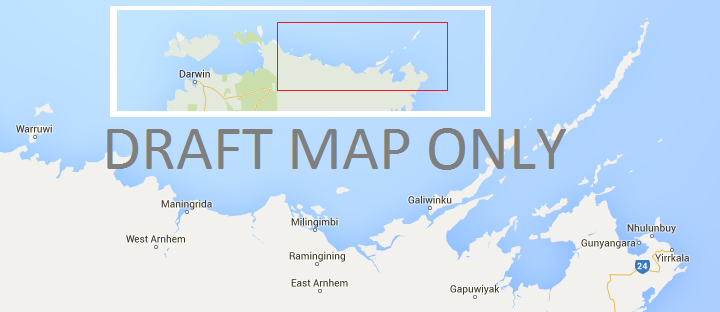
\includegraphics[width=\textwidth]{mapdraft.png}
    \caption[Map showing the study area, NE Arnhem Land]{
        Map showing the study area, NE Arnhem Land.
        Analysis in \autoref{ch:quantify} uses weather observations from several of the towns shown.
        TODO:  better map (inset all Aus), label towns and referenced place names
        (Elcho Island, etc.)
        Would also be good to shade by Indigenous group, approximately.
        }
    \label{fig:arnhem-map}
\end{figure}

TODO:  need better description of location (relative to whole continent and within AL).

This study focusses on North-East Arnhem Land, particularly Elcho Island
and the town of Galiwinku.  Figure~\ref{fig:arnhem-map} shows the study area.
Qualitative seasonality is described for Galiwinku and Milingimbi;
quantitative weather observations are from Waruwi, Maningrida, Milingimbi,
Galiwinku, and Nhulunbuy.

These sites are all in Yolngu country, in the Anrhem Coast bioregion \citep{ens2014}.
The landscape is dominated by tropical woodland, from mangroves on the coastline 
through dense forest to more open woody grasslands further inland.

~\\

TODO:  also need to outline the temporal scale I'm dealing with - recent
decades for both qualitative and numerical data.


Yolngu have a tradition of engagement across cultures, including
the Macassan trade with Indonesia in the 1700s and engagement with Methodist
missionaries throughout the 1900s.

% RELEVANCE UNCLEAR; REVISE BARK PETIION REFERENCES
The Yirrkala Bark Petition (\autoref{fig:bark-petition}) marks a crucial
point in the Australian land rights movement, recognised by indigenous and
non-indigenous people alike.  It is also prone to misinterpretation by those
who see a document in two languages with a decorative border: the border
is the most important part!  (see caption, expand this section)


\begin{wrapfigure}{R}{0.5\textwidth}
    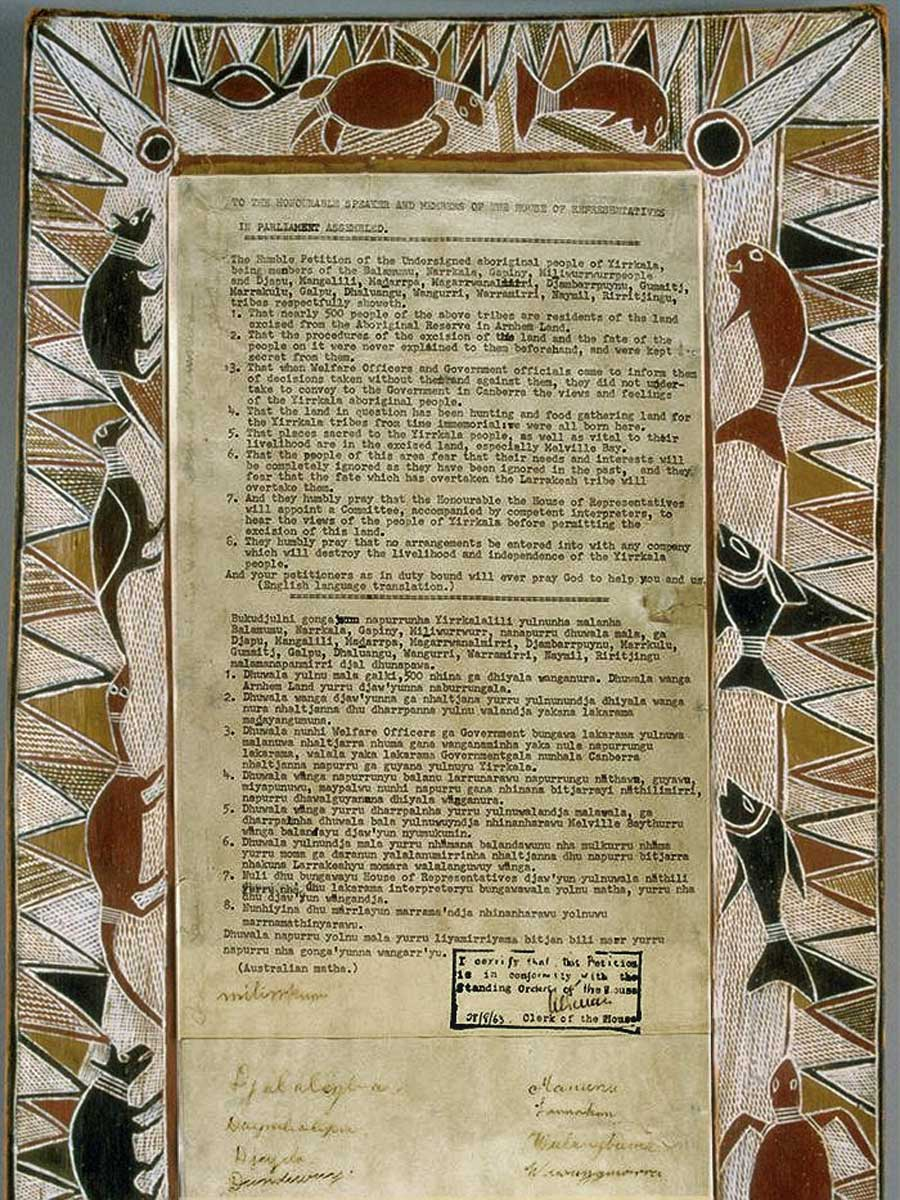
\includegraphics[width=\linewidth]{bark-petition.jpg}
    \caption[The Yirrkala Bark Petition]{
        The Yirrkala Bark Petition, 1963.
        The Bark Petition concerns the bauxite mining lease granted at Nhulunbuy
        without consultation with Yolngu, and helped kick-start the Australian
        land rights movement.

        The petition is presented in three ways: text in English,
        text in Yolngu Matha, and in the border.
        This painting is not a decoration; it is a reproduction of
        the title deeds to the ancestoral estates of the signatories -
        and the most important part of the document.
        }
    \label{fig:bark-petition}
\end{wrapfigure}


In a letter inviting collaboration on this research (see \autoref{sec:ethics}),
a senior Yonlgu man explained that:

\blockquote{
    For Yolngu (the people of North Eastern Arnhem Land) it is the Liyagadhaman
    who carry within them the wisdom and knowledge of these matters.
    It is right that in this research you have approached me to talk about these
    things. I can also introduce you to others who have this knowledge.  ...

    Yolngu have made careful observation of the ways of nature and the seasons
    over the millennia and have passed on that knowledge down the generations.
    We know the changes that are taking place in the seasons and I am willing
    to talk with you about what I have seen happening around me.
}




The BOM describes the 
climate as ``hot and humid'', with daytime temperatures between 25 and 40 
degrees year-round.  Rainfall and humidity are dominated by monsoon 
seasonality, and the seasons are commonly described by non-indigenous residents 
as “the Wet” and “the Dry” – though after a few years living in the tropics
many also recognise “the Buildup” of pre-wet humidity \citep{willmett2009}.

The key meteorological determinants of seasonality are temperature (especially 
night-time), rainfall, humidity, and wind strength and direction.  The annual 
cycle is driven primarily by the Indian Ocean monsoon.  The seasonal effect of 
temperature is felt most strongly at night, as daytime temperatures are very 
consistent and the latent heat of available water has a strong effect.

However, wet/dry/buildup misses important nuance in the seasonality of the 
area.  \autoref{fig:yolngu-seasons} shows one summary of Yolngu seasonality,
with significantly more seasons.  \citet{woodward2012b} notes
\blockquote{
    four factors that interconnect within each of the seasonal
    knowledge systems; a focus on resource use, knowledge of complex
    ecological indicators to facilitate resource collection,
    knowledge of meteorological phenomena and a strong
    metaphysical/spiritual understanding.
}



\section{Thesis Structure}

The chapters of this thesis follow the conventional structure for a scientific
report, and are largely self-describing - Introduction, Literature Review,
Methods, Results, Discussion, and Conclusion.

TODO - outline content of each and justify section-level structure.
Include pointers to unusual structure, eg literature spread out.

~\\

Interdisciplinary methods occur throughout, and are particularly important
to the methods, results, and discussion.  These chapters are divided into
sections which focus on each approach used to investigate seasons:
qualitative research with Indigenous participants,
quantitative meteorological descriptions,
combining diverse perspectives, and
a summary which synthesises these aspects.

Note that while the literature review provides a general overview,
other chapters reference specific literature where relevant to e.g.
results, if it would not fit in the general review.

The division of chapters into sections
reflects the methodology of distinct steps that are
later extended.  The academic and local context provides direction and focus
for the qualitative research.  In turn, the qualitative data and context
allows construction of a bridge to quantitative data and methods.



\section{Scoping and Delimitations}
TODO - integrate scope and delimitations to avoid a positive/negative distinction.

My guiding research questions are:
\begin{itemize}
\item How are Yolngu seasonal calendars defined, and does this vary?
\item Which Yolngu calendar is best suited for mixed-methods study?
\item What are the properties and changes that define this calendar?
\item How may these seasons be characterised by meterological parameters?
\end{itemize}



~\\

The constraints of an Honour thesis mean that there are also many things
that are \emph{not} covered.  ADD MORE DELIMITATIONS
%
Go back to mid-year review to fill out list; then re-write as paragraph
%
\begin{itemize}
\item Historical understandings or events are out of scope, beyond those
        in the observational record (~1970-present) and within living memory.
\item All interviews were conducted in English, and likely lost some nuance.
\item Was unable to go on-country due to resource constraints; spoke in Darwin.
\item Small sample pool and unable to revisit.
\item Far more depth in concepts of what a season is than I could explore.
\item etc... there's a lot more.
\end{itemize}




